\chapter{Technische Implementierung der Algorithmen}
	\label{Implementierung}
	\section{Kurze Einführung in die Programmiersprache und Programmierumgebung}
	
		Für die Implementierung der Wegfindung wurde im Abschnitt \ref{Aufgabenstellung_Pathfinding} definiert, dass diese auf einer Siemens \ac{SPS} (englisch: \ac{PLC})  der S7-1200er Reihe lauffähig sein muss. Bei der 1200er Reihe handelt es sich um  Steuerungen des niedrigen Leistungssegments. Für die Projektierung und Programmierung von Anlagen mit Steuerungen dieser Art wird deine proprietäre Entwicklungsumgebung namens \ac{TIA-Portal} von Siemens zur Verfügung gestellt.
		
		\subsection{Siemens TIA-Portal}
		
			Das Siemens \ac{TIA-Portal} vereinigt viele Aspekte der Projektierung von Anlagen in einer einheitlichen Oberfläche. Innerhalb des \ac{TIA-Portal}s können beispielsweise Projekte bestehend aus mehreren Antrieben und \ac{SPS}en gemeinsam geplant und erstellt werden. Das  \ac{TIA-Portal} ist aktuell in der Version 13 verfügbar und bietet vor allem eine anwenderfreundliche Oberfläche für komplexe Automatisierungsaufgaben. Die Kernkomponente für die Erstellung von Programmen für \aclp{SPS} ist die Programmierumgebung \acs{STEP7}\footnote{\ac{STEP7}}. Abbildung \ref{Projektansicht} zeigt die Projektansicht des \ac{TIA-Portal}s.
			
			\begin{figure}
				\centering
				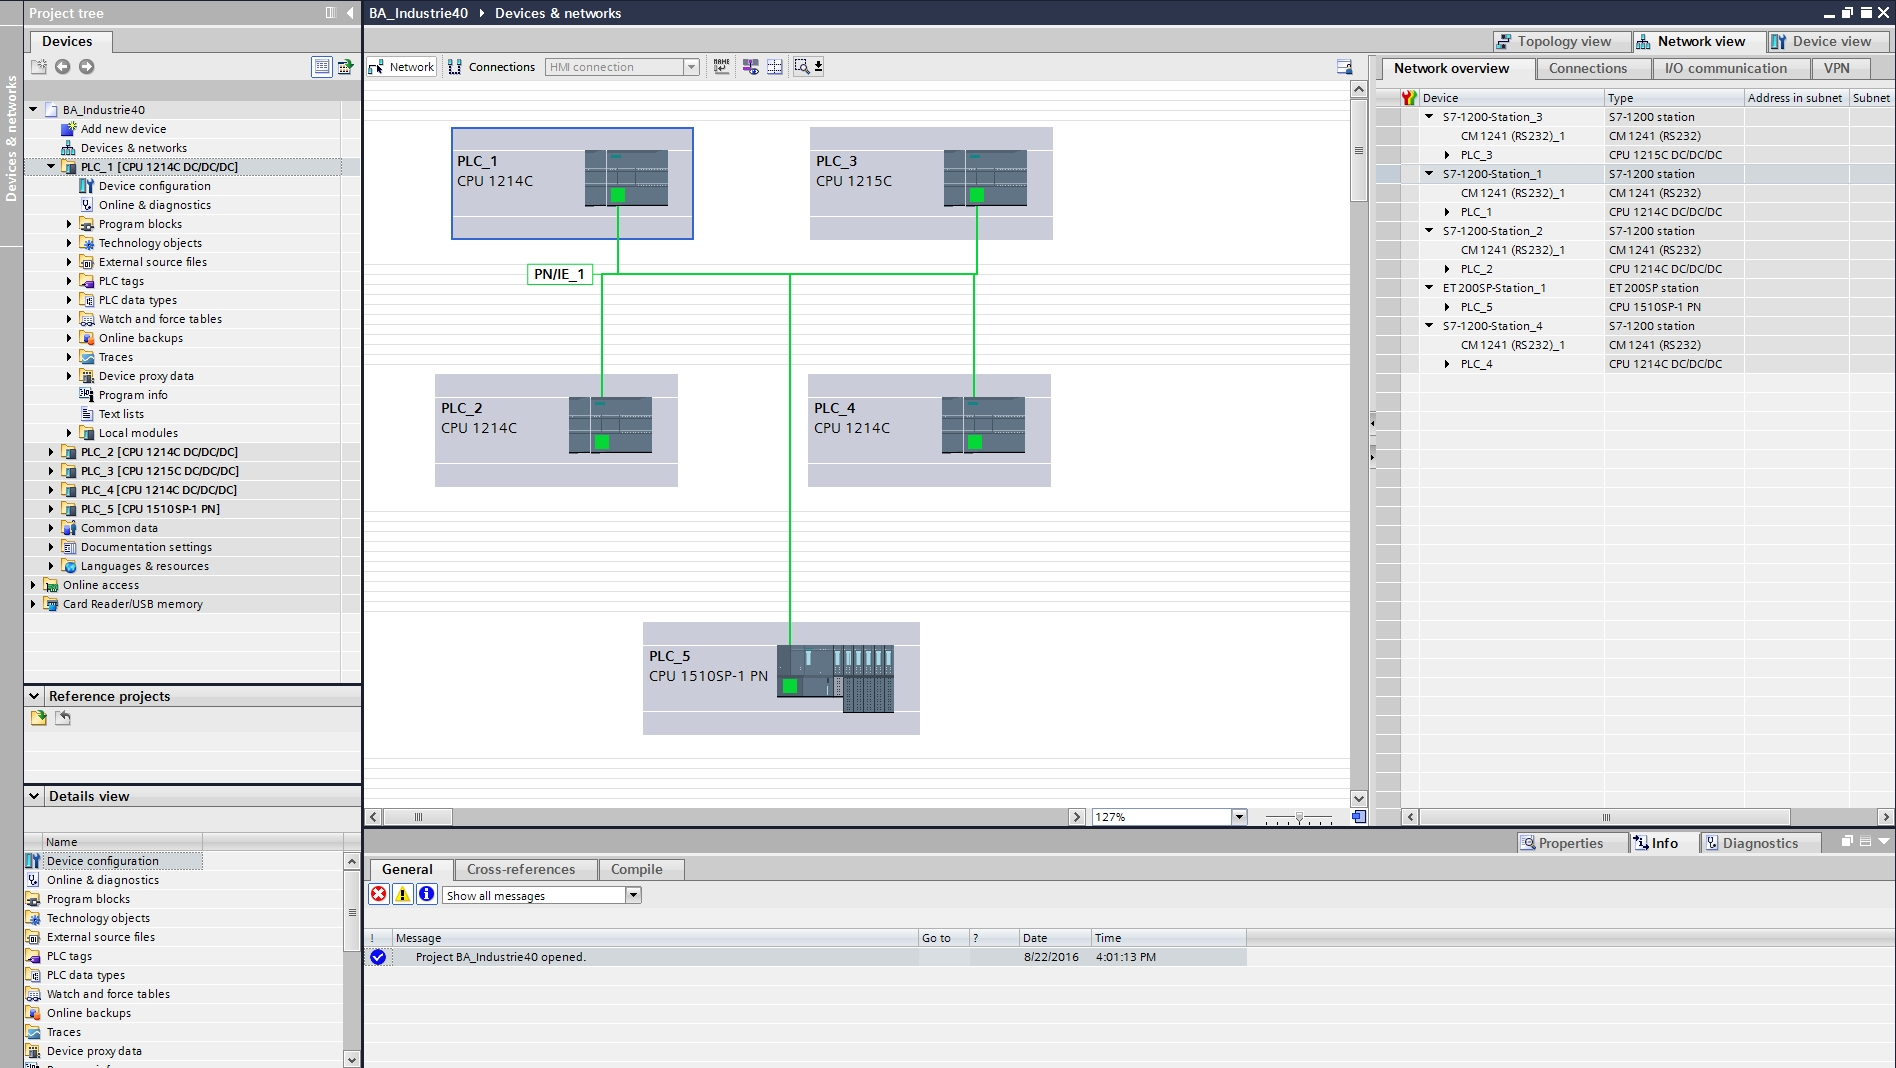
\includegraphics[scale=0.25]{/Bilder/TIA-Portal_Projektansicht}
				\vspace{0.2cm}
				\caption{Projektansicht des \ac{TIA-Portal}s.}\label{Projektansicht}
			\end{figure}
			
		
		\subsection{Programmierumgebung STEP7}
			Die Grundelemente eines \ac{STEP7}-Projekts sind die projektierten Steuerungen. Diese sind wiederum unterteilt in Teilelemente wie die Hardware-Konfiguration der Steuerung, das Anwenderprogramm, die verwendeten Variablen, benötigte Datentyp-Definitionen und Komponenten zur Überwachung und Modifizierung der Steuerungsdaten im laufenden Betrieb. Für die Implementierung der Wegfindungsalgorithmen sind vor allem das Steuerungsprogramm und die darin verwendeten Datentypen von Bedeutung. Ein Anwenderprogramm besteht aus bis zu vier Arten von Programmbausteinen \cite{STEP7Prog}:\\
					
			
			\begin{longtable}{{p{4.5cm} p{10cm}}}
				
				\textbf{\ac{OB}:} & Diese Bausteine bilden die Schnittstelle zwischen dem Betriebssystem der Steuerung und dem Anwenderprogramm. Sie haben jeweils vordefinierte Funktionalitäten und bilden somit das Grundgerüst des Anwenderprogramms. Die in dieser Implementierung verwendeten \ac{OB}s sind zum einen der Systemstart-Baustein sowie Bausteine zur zyklischen Abarbeitung von Teilschichten des Programms.\\[0.5cm]
				\textbf{\ac{DB}:} & Datenbausteine dienen zur Speicherung von variablen Daten, auf die von dem gesamten Anwenderprogramm  aus zugegriffen werden kann. Sie werden unter anderem zur Sicherung der Topologiedaten der Anlage, sowie als Schnittstellen zwischen verschiedenen Programmschichten verwendet.\\[0.5cm]
				\textbf{\ac{FC}:} & Funktionen sind Bausteine zur elementaren Kapselung von Funktionalitäten. Sie werden im Anwenderprogramm definiert als Unterprogramme, die keinen eigenen Speicher zur Sicherung von Variablenwerten zwischen zwei aufeinanderfolgenden Programmaufrufen benötigen.\\[0.5cm]
				\textbf{\ac{FB}:} & Funktionsbausteine realisieren wie \ac{FC}s Unterprogramme, stellen aber zusätzlichen Speicherbereich für die permanente Sicherung von internen Variablen zur Verfügung. Bei der Verwendung eines \ac{FB}s wird bei dessen Initialisierung ein entsprechender Instanz-\ac{DB} generiert, in welchem Daten für die Verwendung in späteren Programmaufrufen gespeichert werden können.\\[0.5cm]
				
			\end{longtable}
			
			\begin{figure}[h]
				\centering
				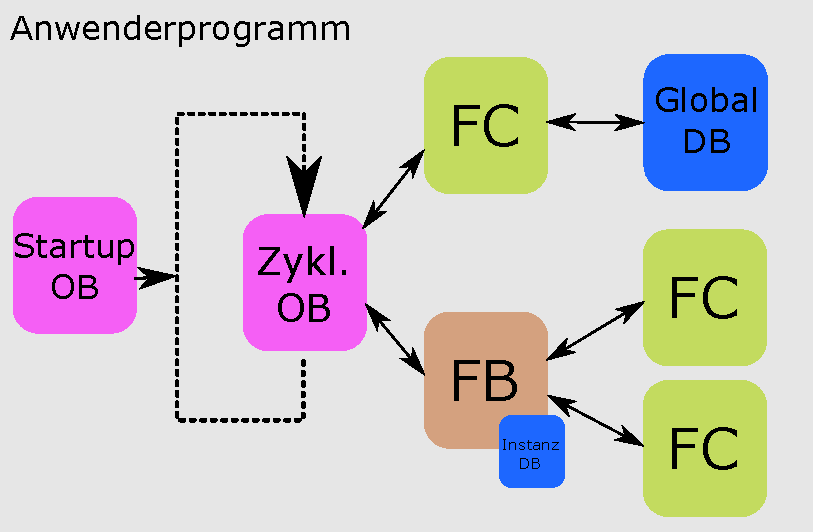
\includegraphics{/Bilder/AnwenderprogrammDarstellungPDF}
				\vspace{0.2cm}
				\caption{Beispielhafter Aufbau eines Anwenderprogramms.}\label{Anwenderprogramm Darstellung}
			\end{figure}
			
			\ac{FC}s und \ac{FB}s entsprechen den Funktionsdefinitionen in anderen Programmiersprachen. Es können die Schnittstellen der Bausteine sowie deren Schnittstellentypen definiert werden. IN-Variablen werden beispielsweise nur lesend verwendet, OUT-Variablen werden nur schreibend und INOUT-Variablen werden sowohl schreibend als auch lesend verwendet. Innerhalb eines Bausteins können zum einen temporäre als auch statische\footnote{persistent über Funktionsaufrufe hinaus.} Variablen zur Zwischenspeicherung von Variablenwerten während der Programmabarbeitung genutzt werden. Da statische Variablen einen Instanz-\ac{DB} benötigen, sind sie nur in \ac{FB}s verwendbar.
			\\[4pt]
			Die Bausteine können in einer von vier Programmiersprachen geschrieben werden. \ac{FUP} und \ac{KOP} sind Sprachen zur graphischen Programmierung. \ac{AWL} ist eine Assembler-ähnliche Sprache für generelle Programmieraufgaben, welche unter anderem die byteweise Manipulation von Daten vereinfacht. \ac{SCL} ist eine Pascal-ähnliche Programmiersprache, die durch ihre einfachen Implementierungsmöglichkeiten von Schleifen geeignet ist für die Programmierung komplexer Aufgabenstellungen. Bei der Erstellung des Anwenderprogramms für die Wegfindung wurden die verwendeten \ac{OB}s in \ac{FUP} erstellt und alle anderen Bausteine in SCL. Die Abbildung \ref{Vergleich FUPSCL} zeigt den unterschiedlichen Aufbau der beiden Programmiersprachen.
			
			\begin{figure}[h]
				\begin{center}
					\subfigure[FUP]{\label{Sample FUP}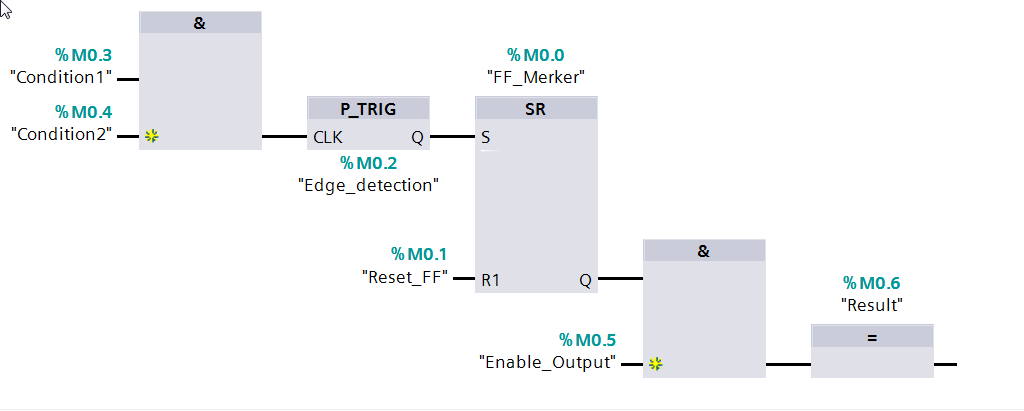
\includegraphics[scale=0.3]{/Bilder/SampleFUP}}
					\subfigure[SCL]{\label{Sample SCL}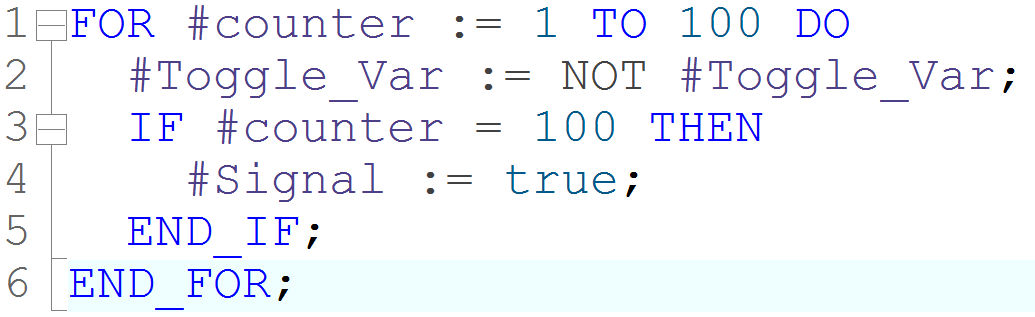
\includegraphics[scale=0.3]{/Bilder/SampleSCL}}
				\end{center}
				\caption{Vergleich der Programmiersprachen FUP und SCL.}\label{Vergleich FUPSCL}
			\end{figure}
			
		%\subsection{SCL}
	
		\subsection{Arbeitsweise einer SPS}
			
			Eine \acl{SPS} arbeitet nach dem Prinzip eines Echtzeitsystems. Das projektierte Anwenderprogramm wird in einer Endlosschleife zyklisch abgearbeitet. Zu Beginn eines Bearbeitungszyklus wird ein Prozessabbild aller Eingangsbaugruppen  der Steuerung generiert, welches für den kompletten Zyklus als Basis für die Werte der Eingänge genutzt wird. Während der Zyklusabarbeitung werden die berechneten Werte für die Ausgänge in ein weiteres Prozessabbild geschrieben, welches erst nach Ende des aktuellen Bearbeitungszyklus an die Ausgangsbaugruppen übertragen wird. Somit müssen Mehrfachzuweisungen innerhalb eines Zyklus vermieden werden, da nur die letzte Zuweisung an die Ausgänge weitergegeben wird. Durch \ac{OB}s können zusätzliche Funktionen außerhalb der zyklischen Bearbeitung realisiert werden. Beispielsweise können im Startup-\ac{OB} einmalig Anweisungen beim Hochfahren der CPU ausgeführt werden.
	
	\section{Realisierung der Anlagentopologie}
		
		Als Grundlage für die Wegfindung muss zunächst die Anlage definiert werden. Wie bereits in Abschnitt \ref{Graph_Anlage} beschrieben, wird die Anlage durch einen Graphen mit positiven Kantengewichtungen dargestellt. Für die technische Realisierung der Anlage ist unter anderem wichtig, dass die Beschreibung der Topologie erweiterbar ist, und sich der physikalische Aufbau leicht umsetzen lässt.
		
		\subsection{Gewählte Anlagentopologie}
			
			Im Hinblick auf die in Abschnitt \ref{Ziele_Wegfindung} definierten Implementierungsstufen und die dazu gehörigen Use-cases wurde für die Topologie der Anlage eine Matrixstruktur gewählt.  Bei der Platzierung der Bearbeitungsstationen an die Außenkanten der 2x4 Wabenstruktur können die Fahrstrecken im Inneren als eine Art Überholspur für Fahrzeuge genutzt werden, die sich schneller durch die Anlage bewegen. Zudem wurden Eingangs- und Ausgangsknoten als Start und Endpunkt für die Wegfindung definiert. Als zusätzliche Rückführstrecke für Fahrzeuge nach Beendigung ihres Bearbeitungsauftrags wurde eine Rückführstrecke von dem End- zum Startknoten der Anlage hinzugefügt, welche aber in der Wegberechnung nicht berücksichtigt wird. Der Gesamtaufbau der Anlage wird in Abbildung \ref{Schema Strecke} schematisch dargestellt.
			
			\begin{figure}[h]
				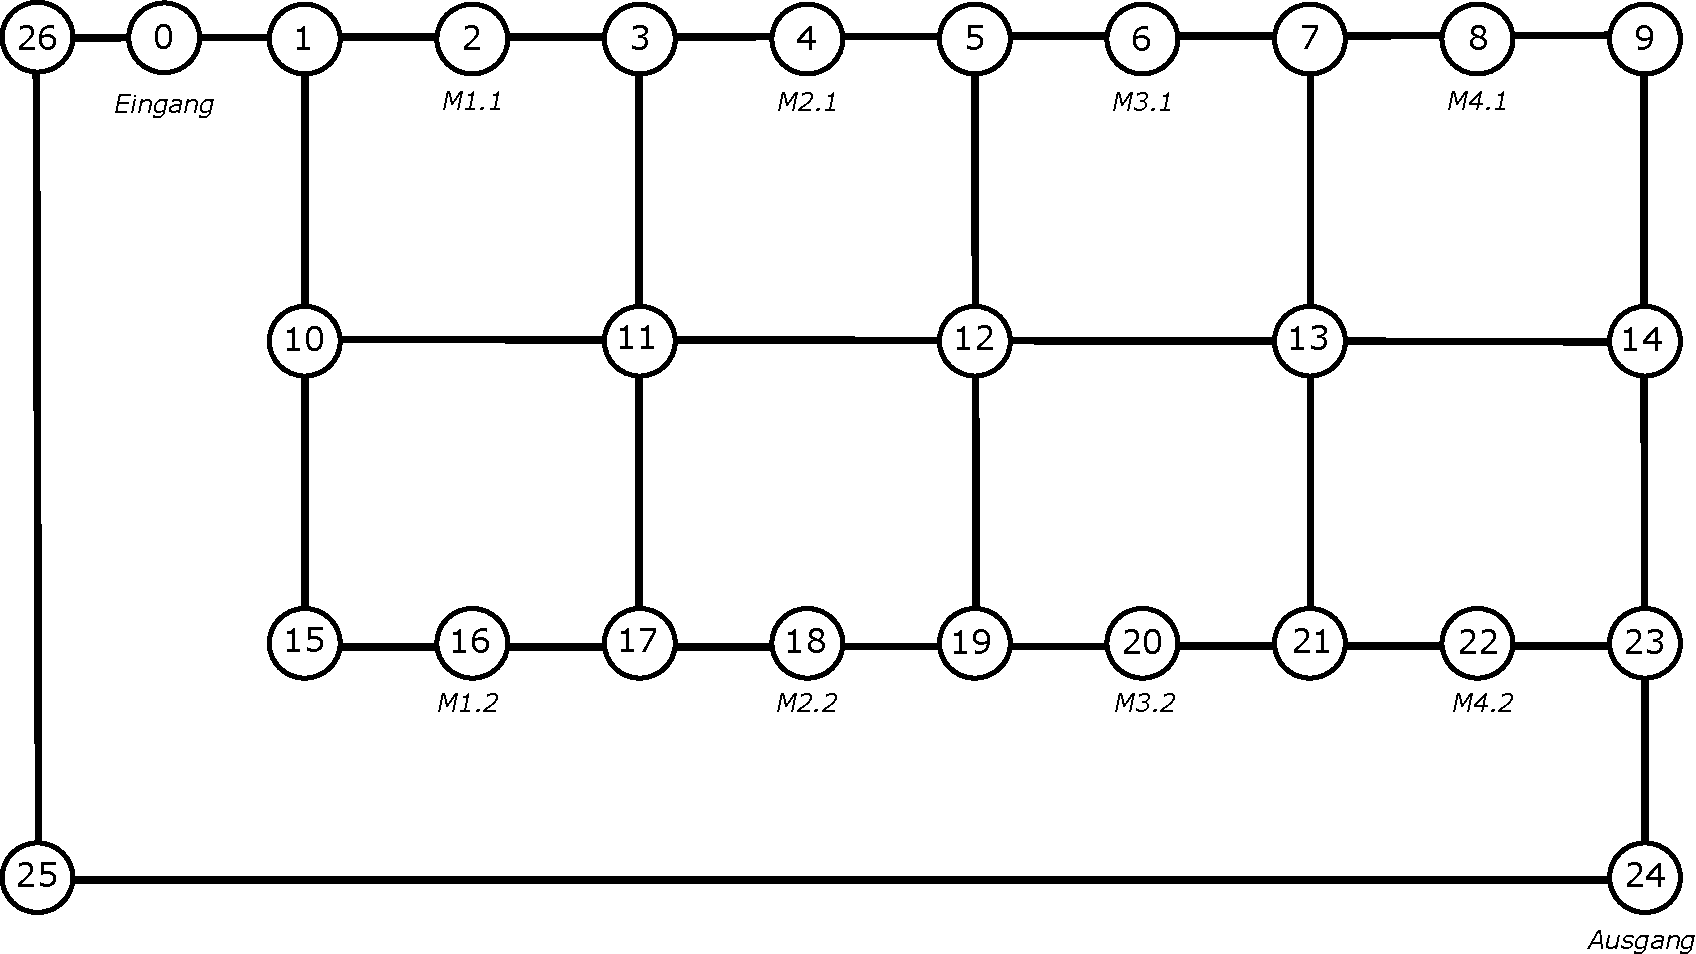
\includegraphics[scale=0.5]{/Bilder/SchemaStreckePDF}\\
				\caption{Schematische Darstellung der Strecke. Die Zahlen repräsentieren die KnotenIDs.}\label{Schema Strecke}
			\end{figure}
		
		\subsection{Physikalischer Aufbau}
			\label{Phys_Anlage}
			In Abschnitt \ref{Alg._Aufgabenstellung} wurde dargelegt, dass die Anlage als Vorführmodell für Konzepte von Industrie 4.0  verwendet werden soll. Somit ist die Portabilität der Anlage ein wichtiger Punkt. In Zusammenarbeit mit Herrn A. Meier wurde als Basis der Anlage ein modulares System aus leichten Kartonplatten ausgewählt. Aufbauend hierauf wurden für die optische Sensorik der Fahrsteuerung die Fahrstrecken mit dunklem Isolierband aufbracht. Diese lassen sich bei Bedarf auch entfernen oder modifizieren, um Änderungen der Anlagentopologie zu simulieren. Die Kreuzungen der Fahrstrecken, die die Entscheidungspunkte für die Fahrzeugsteuerung und die Wegfindung darstellen, entsprechen den Knoten des korrespondierenden Anlagengraphen. Die Fahrstrecken, als Verbindungen zwischen einzelnen Entscheidungspunkten, entsprechen somit den Kanten des Graphen.
			
			\begin{figure}[h]
				\centering
				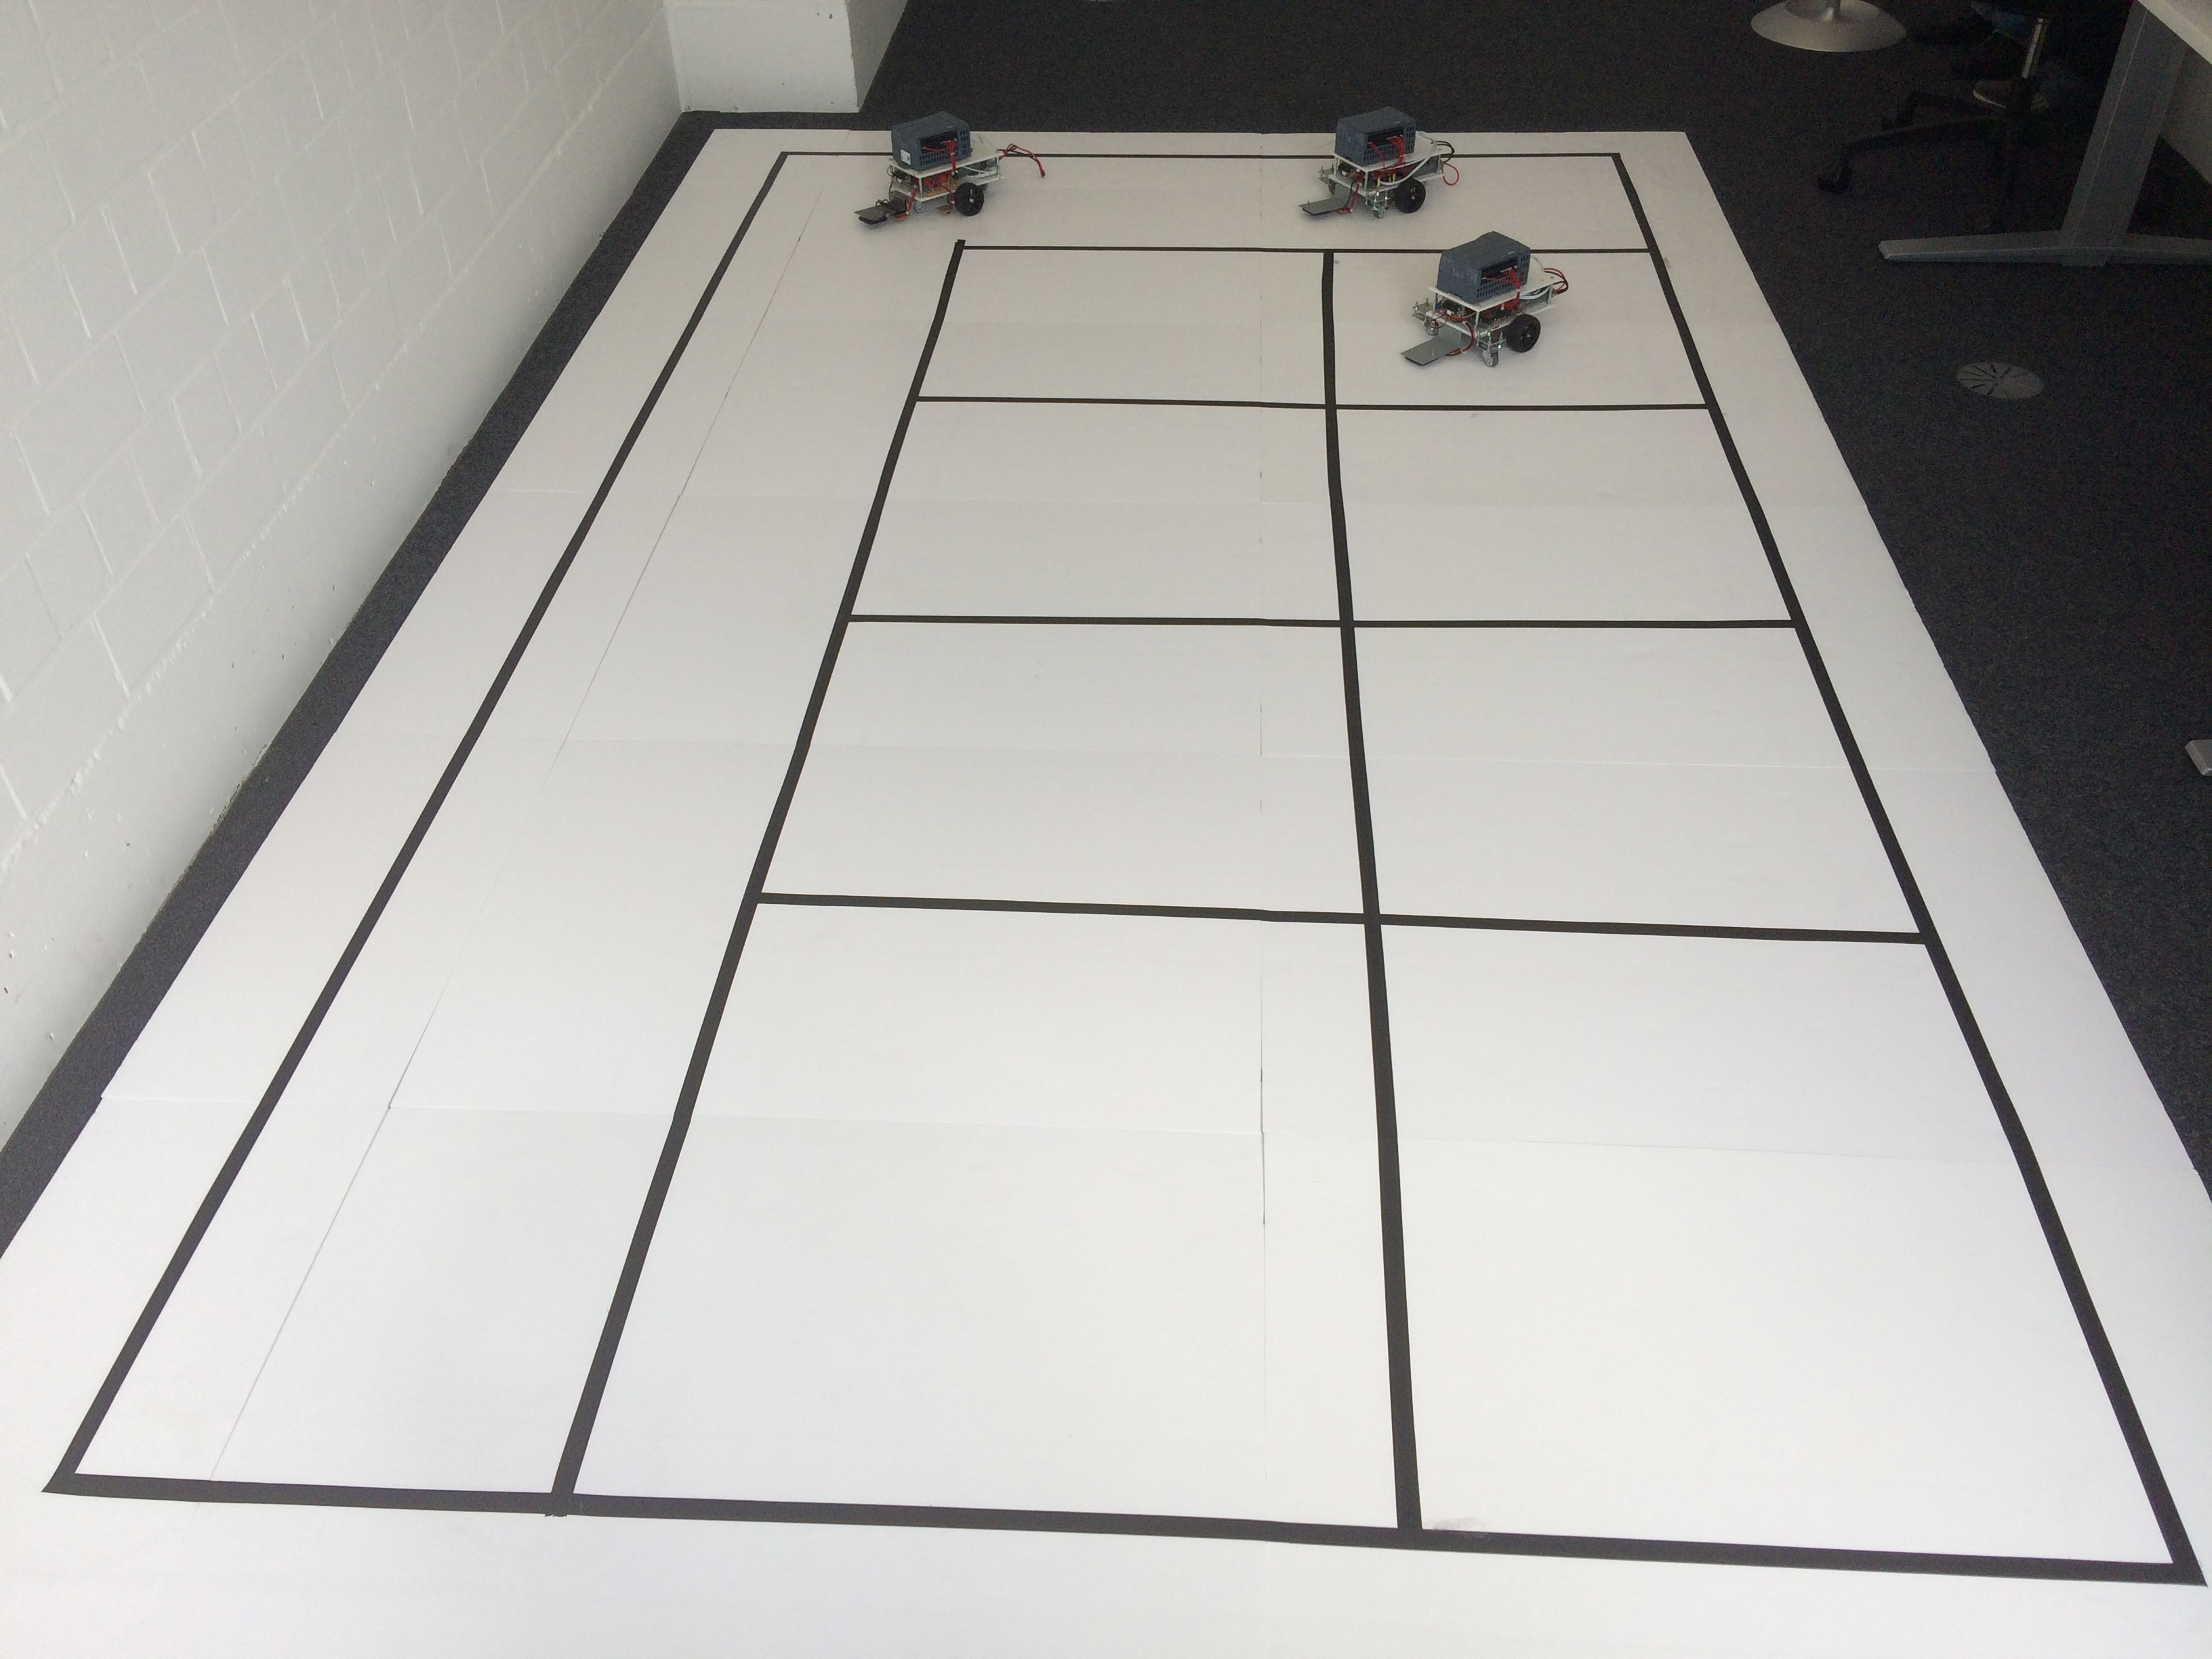
\includegraphics[scale=0.125]{/Bilder/PhotoStreckeSeite}\label{Photo Strecke}
				\vspace{0.2cm}
				\caption{Bild der realisierten Anlage \cite{Meier16}, aufgenommen von der Ausgangsseite.}
			\end{figure}
			
			Für die Wegfindung ist es zudem wichtig die aktuelle Position eines Fahrzeugs ermitteln zu können, um diese als Basis für den Startknoten der Berechnung benutzen zu können. Aus diesem Grund wurden unterschiedliche Methoden zur Orientierung der Fahrzeuge innerhalb der Anlage untersucht. Da eine zentrale Erfassung der Fahrzeugpositionen durch zusammengeschaltete mechanische, analoge oder optische Sensoren nicht in das Konzept der Dezentralisierung von Industrie 4.0 passt, wurde ein \ac{RFID}-basiertes Identifikationssystem für die Positionserfassung ausgewählt. Dieses funktioniert durch die Anbringung von \ac{RFID}-Transpondern auf der Unterseite der Kartonplatten, jeweils auf Höhe eines Entscheidungsknotens. Jedes Fahrzeug besitzt einen \ac{RFID}-Sensor, welcher vor dem Fahrzeug an einem Ausleger befestigt ist, um Anlagenknoten zu identifizieren, an die sich das Fahrzeug annähert. Hier hat sich die Entscheidung für Kartonplatten zur Anlagenmodellierung als Vorteil erwiesen, da die Transpondersignale auch durch den Karton auf der Oberseite der Anlagenplatten detektierbar ist, und die Transponder somit nicht auf der Fahrstrecke selbst befestigt werden müssen, was zu Behinderungen beim Fahren führen könnte.
			
		\subsection{Beschreibung als Knotenliste}
			\label{Knotenliste}
			Sowohl für die Wegfindung als auch für die Fahrsteuerung wird eine digitale Repräsentation der Anlage benötigt. Aufgrund der einfachen Erweiterbarkeit wurde hier die Darstellungsform der Knotenliste für Graphen ausgewählt, da bei dieser Datenstruktur einfach Knoten hinzugefügt und entfernt werden können. Für einen Einzelknoten wurde die Anzahl der möglichen Kanten pro Knoten auf vier beschränkt. Dies macht eine Zuordnung der einzelnen Kanten zu den vier Himmelsrichtungen möglich. Dies wird vor allem für die Fahrsteuerung benötigt, da hier eine der Anforderungen die Möglichkeit der Ausführung von 90-Grad-Kurven ist. Da die Fahrsteuerung als getrenntes Programmmodul implementiert wurde besitzt sie eine Kopie der Knotenliste der Anlage mit den zusätzlichen, bei der Wegfindung nicht benötigten Knoten der Rückführstrecke.
			Ein Einzelknoten hat folgenden generellen Aufbau:\\
			
			\begin{table}[h]
			
				\begin{tabular}{| l | l | l |}
					
					\hline
					\textbf{ID} &
					\multicolumn{2}{c|}{Nummer des aktuellen Knoten} \\[1pt]
					\hline
					\multirow{8}{*}{Kanten}
						& ID Nord & verbundener Knoten in Richtung Norden \\[1pt] \cline{2-3}
						& Dist. Nord & Abstand zum Knoten in Richtung Norden\\[1pt] \cline{2-3}
						& ID Ost & verbundener Knoten in Richtung Osten \\[1pt] \cline{2-3}
						& Dist. Ost & Abstand zum Knoten in Richtung Osten\\[1pt] \cline{2-3}
						& ID Süd & verbundener Knoten in Richtung Süden\\[1pt] \cline{2-3}
						& Dist. Süd & Abstand zum Knoten in Richtung Süden\\[1pt] \cline{2-3}
						& ID West & verbundener Knoten in Richtung Westen\\[1pt] \cline{2-3}
						& Dist. West & Abstand zum Knoten in Richtung Westen\\[1pt] 
						\hline
				
				\end{tabular}
				\vspace{0.2cm}
				\caption{Aufbau eines Topologieknotens.}
			\end{table}
			
			Da in \ac{STEP7} Speicher nicht dynamisch alloziert werden kann, hat jeder Knoten immer Speicherplatz für die Daten von allen vier möglichen Kanten, auch wenn er in der realen Anlage mit weniger als vier Knoten verbunden ist. Da die ID "`0"' für den Startknoten reserviert wurde, werden Verbindungsrichtungen durch eine "`-1"' im ID-Feld als nicht verbunden gekennzeichnet. Hierdurch wird auch der zugehörige Abstand ignoriert.
			\\[4pt]
			Die Datenstruktur der Knotenliste selbst besteht aus einem einfachen Array mit Einzelknoten als Arrayelementen. Dieses Größe dieses Arrays wird initialisiert mit einer Konstanten, welche die Gesamtanzahl der möglichen Anlagenknoten enthält. Zusätzlich zu dem Knotenarray besteht der Listendatentyp noch aus der Anzahl der wirklich im Array enthaltenen Knoten. Diese wurde aus Gründen der Konsistenz hinzugefügt , da andere selbst definierte Listentypen im Projekt mit variablen Anzahlen von Arrayelementen arbeiten, was bei der Anlagentopologie nur selten der Fall ist. Dies könnte in diesem Falle genutzt werden wenn zu einem späteren Zeitpunkt weitere Knoten zur Anlage hinzugefügt werden. Hier muss aber ein Neustart des \ac{FTF} durchgeführt werden, da sonst die in Abschnitt \ref{Verwendung_Alg} besprochene Heuristik-Berechnung für die neu hinzugefügten Knoten nicht existiert und somit die Knoten nicht für die Wegberechnung verwendet werden können.
			\\[4pt]
			Abschließend sei noch erwähnt, dass die in Abschnitt \ref{Phys_Anlage} angesprochenen \ac{RFID}-Werte der Knoten nicht für die Wegfindung relevant sind. Das Einlesen und die Zuordnung von \ac{RFID}s zu den entsprechenden Knoten wird komplett in der Fahrzeugsteuerungsschicht erledigt, welche der Wegfindungsschicht dann nur die interne KnotenID weitergibt.
			
		\subsection{Beschreibung als Adjazenzmatrix}
			\label{Adjazenzmatrix}
			Unter dem Aspekt der Erweiterbarkeit ist die Listendarstellung des Graphen ideal, da Knoten unabhängig von ihrer Position innerhalb der Anlage einfach am Ende der Liste angehängt werden können. Solange der neue Knoten gültig ist, kann der erweiterte Anlagengraph verwendet werden. Für die eigentliche Wegfindung ist eine solche Liste jedoch ungünstig, um schnell den Abstand eines Knotens zu einem beliebigen anderen Knoten zu prüfen. Bei einer Liste müsste im schlechtesten Fall bei Überprüfung des zuletzt hinzugefügten Knotens das komplette Array durchlaufen werden. Aus diesem Grund wird beim Hochfahren der CPU, vor der Berechnung der Heuristik mittels Dijkstra, die Knotenliste geparst und eine Adjazenzmatrix der Anlage generiert. Hier kann in konstanter Zeit\footnote{Aufwand $\mathcal{O}(1)$} der Abstand zwischen zwei Knoten $x$ und $y$ ermittelt werden, indem einfach der in der Matrix unter den Indizes $(x,y)$ hinterlegte Wert abgerufen wird. Dies beschleunigt vor allem die Laufzeit des im zyklischen Betrieb ausgeführten A*-Algorithmus. Für die Berechnung der Heuristiken ist dies weniger von Bedeutung, da hier keine Zeitbeschränkungen vorliegen und nur der weniger kritische Aspekt der kürzeren Hochfahrzeit der \ac{SPS} beeinflusst wird.
			
			\begin{figure}
				\centering
				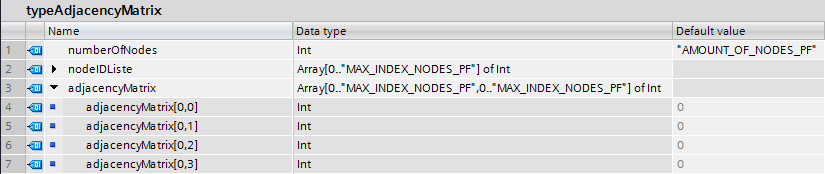
\includegraphics[scale=0.7]{/Bilder/TIA_AdjazenzmatrixDatentyp}
				\vspace{0.2cm}
				\caption{Definition des Datentyps für die Adjazenzmatrix in \ac{STEP7}}
			\end{figure}

	\section{Implementierung der Algorithmen}
		
	
		Das gesamte Programm wurde in einzelne funktionale Schichten aufteilt, um den Industrie 4.0 Aspekt der Modularisierung zu entsprechen. Somit macht es keinen funktionalen Unterschied, ob die Wegfindungsschicht tatsächlich auf derselben Steuerung läuft wie die Fahrzeugsteuerungsschicht.
		\begin{wrapfigure}{r}{5cm}
			\centering
			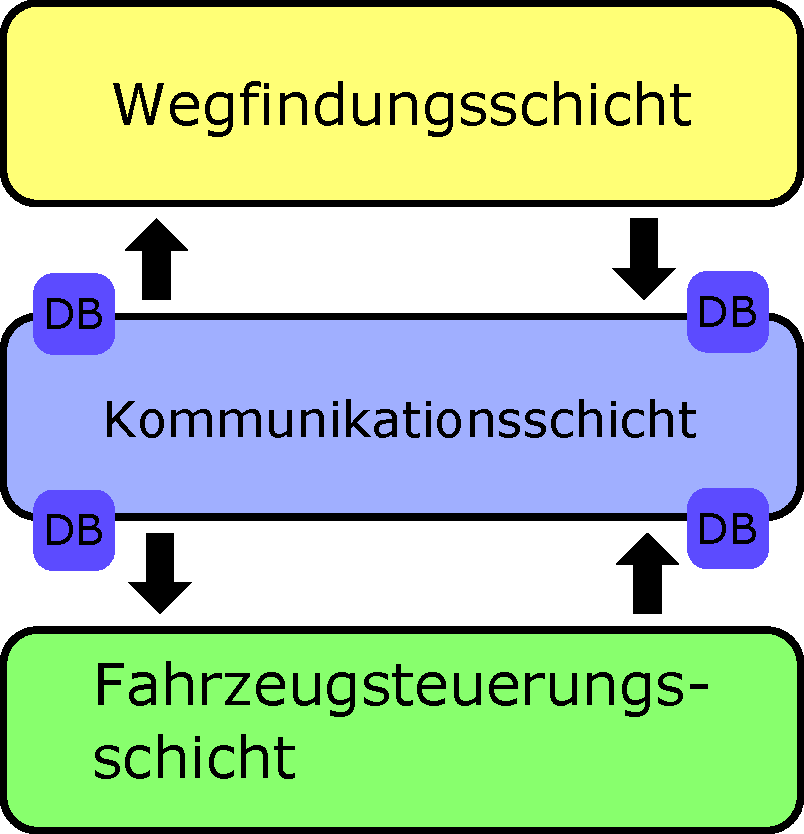
\includegraphics[width= 4.5cm]{/Bilder/BasisSchichtenPDF}
			\vspace{0.2cm}
			\caption{Darstellung der Grobunterteilung des Anwenderprogramms.}
		\end{wrapfigure}
		 Als Schnittstelle dienen hier sowohl bei der Wegfindungs- als auch bei der Fahrzeugsteuerungsschicht  Datenbausteine, in welche die zu übertragenden Ergebnisse geschrieben werden. Diese Daten werden durch die in Kapitel \ref{Kommunikation} näher beschriebene Kommunikationsschicht übertragen. Dies hat den Vorteil, dass unterschiedliche Arten der Kommunikation einfach ausgetauscht werden können, ohne die anderen Schichten zu beeinflussen.
		
		Die in Kapitel \ref{Theorie} beschriebenen Algorithmen wurden beide auf ähnliche Weise in \ac{STEP7} implementiert. Für die A* und Dijkstra-Algorithmen wurden jeweils geeignete Datentypen definiert, welche an die Anforderungen der Algorithmen angepasst wurden. Die Implementierung verwendet hier in beiden Fällen eine Priority-Queue auf Basis eines Arrays, um bei der Berechnung den jeweils nächsten "`besten"' Knoten zu identifizieren. Das Array als Grundlage der Prioritätsschlange wurde hier gewählt, da sich die Realisierung in \ac{STEP7} einfacher gestaltet als beispielsweise die eines Heaps. Dafür müssen hier Abstriche bei der Sortiergeschwindigkeit gemacht werden.
		
		\subsection{Berechnungsdatentypen}
			\label{Datentypen_Berechnung}
			Für die Berechnung der Algorithmen wurden Datentypen erstellt, die alle für den Algorithmus benötigten Informationen enthalten. Die Datentypen beschreiben die Knoten einzeln und werden zur Berechnung in eine Priority-Queue eingefügt. Als Ergebnis der Berechnung wird eine geordnete Liste der Einzelknoten ausgegeben. Die Datentypen enthalten folgende Grunddaten:
			\\
			\begin{table}[h]
				\begin{tabular}{| l | l |}
					\hline
					\textbf{NodeID} & ID des betrachteten Knotens\\ \hline
					\textbf{Dist. to Start} & Bisher zurückgelegter Weg\\ \hline
					\textbf{Expected Dist.} & Vorausichtl. Gesamtpfadlänge durch diesen Knoten (nur A*)\\ \hline
					\textbf{ParentID} & Vorgängerknoten\\
					\hline
				\end{tabular}
				\vspace{0.2cm}
				\caption{Aufbau eines Berechnungsknotens in der Priority-Queue.}
			\end{table}
			
			Der bisher zurückgelegte Weg gibt bei der Dijkstra-Implementierung Aussagen darüber, wie weit ein Knoten von einem Startknoten entfernt ist. Wird dieser Startknoten später als Ziel gewählt, so kann der Abstand als Heuristik für A* verwendet werden\footnote{Bei gerichteten Graphen muss zusätzlich die Gegenrichtung betrachtet werden.}. Da jeweils der kürzeste Weg gesucht ist, wird für diese Datenkomponente sowie auch für den voraussichtlichen Gesamtweg der Initialwert auf den Maximalwert des verwendeten Datentyps gesetzt, in diesem Fall 65535 für 16-Bit Integer. Dies entspricht damit einem unendlichen Abstand zu dem Startknoten.
			\\
			\begin{figure}[h]
				\centering
				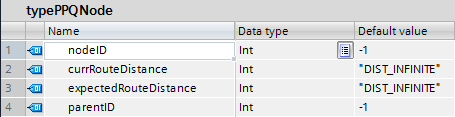
\includegraphics[scale=0.9]{/Bilder/TIA_PPQNodeDatentyp}
				\vspace{0.2cm}
				\caption{Definition des Priority-Queue Wegfindungsknotens in \ac{STEP7}}
			\end{figure}
			\\
			Die voraussichtliche Pfadlänge bei dem Datentyp für den A*-Algorithmus setzt sich zusammen aus dem bisher zurückgelegten Weg und dem geschätzten Wert für den restlichen Weg zum Ziel. Bei Verwendung einer exakten Heuristik ist dieser Wert für alle Knoten auf dem kürzesten Pfad immer konstant, solange sich die Anlage seit Berechnung der Dijkstra-Heuristik nicht verändert hat.
			\\[4pt]
			Der Zeiger zum Vorgängerknoten wurde hier als einfache Zahl implementiert, da das Pointer-Konstrukt in \ac{STEP7} etwas anders funktioniert als beispielsweise in der Programmiersprache C. Dies hat den Nachteil das bei der Zusammenstellung der Route\footnote{beschrieben in Abschnitt \ref{Routengeneration}.} anhand der Knotenliste etwas mehr Zeit verwendet werden muss, da die Liste jeweils nach dem Vorgängerknoten durchsucht wird.
		
		\subsection{Priority-Queue}
		
			Da in \ac{STEP7} keine Container-Datentypen existieren, die mit unterschiedlichen Elementen zurechtkommen, wurden für beide Algorithmen getrennte Datentypen für die Priority-Queue definiert. Diese existieren analog zu der in Abschnitt \ref{Knotenliste} beschriebenen Anlagenknotenliste aus einem Array der Knotenelemente und der Anzahl der beinhalteten Elemente. Dies wurde aus Gründen der Effizienz auf diese Art realisiert, da der große Vorteil des A*-Algorithmus vor allem darin liegt, dass nur ein kleiner Teil der Knoten der Anlage betrachtet werden muss. Da das Array aber nicht dynamisch mit der benötigten Größe alloziert werden kann, sondern immer den schlechtesten Fall berücksichtigen muss, wurde zur Initialisierung des Arrays die Gesamtanzahl der Anlagenknoten als Konstante verwendet. Damit somit bei den Priority-Queue-Operationen nicht die leeren Restplätze des Arrays mit berücksichtigt werden, wurde die Anzahl der Knoten als Datenkomponente mit hinzugefügt. Besteht die Anlage beispielsweise aus 40 Knoten aber es befinden sich nur 6 echte Knoten in der Prioritätsschlange, so laufen alle Schleifen nur über die Elemente null bis fünf.
			\\[4pt]
			Zur Verwendung der Priority-Queue wurden für beide Listendatentypen Zugriffs- und Verwaltungsfunktionen implementiert. \ac{STEP7} besitzt zwar die Möglichkeit Funktionen mittels eines sogenannten VARIANT-Pointers so zu implementieren, dass sie analog zum Konzept der Überladung bei Objektorientierter Programmierung mit unterschiedlichen Eingangsdatentypen zurechtkommen\cite{STEP7Prog}, dies ist in diesem Fall aber nicht möglich, da nicht effizient\footnote{es können nicht Elemente sondern nur Datenbereiche adressiert werden.} auf die Einzelelemente des Datentyps zugegriffen werden kann. Aus diesem Grund wurden die folgenden Operationen für jeden der beiden Datentypen implementiert:
			
			\begin{itemize}
				\item \textbf{Insert}: Einfügen eines Knotens in die Priority-Queue.
				\item \textbf{Pop}: Ausgabe und Entfernung des nach der Prioritätsbedingung "`besten"' Knotens aus der Priority-Queue.
				\item \textbf{Sort}: Wiederherstellung der Prioritätsschlangeneigenschaften durch Sortierung.
				\item \textbf{Contains}: Überprüfung, ob Knoten bereits in der Schlange enthalten ist.
				\item \textbf{UpdateNode}: Modifizierung eines Knotens in der Priority-Queue.
			\end{itemize}
			
			Die Operationen "`Insert"', "`Pop"' und "`UpdateNode"' beinhalten alle eine abschließende Wiederherstellung  der Prioritätsbedingung mittels der in \textbf{INSERT CODE REFERENCE HERE} dargestelten "`Sort"'-Funktion.\\
			Um die Zugriffsoperationen effizienter zu machen, wurden die Prioritätsschlangen so implementiert, dass das beste Element der letzte gültige Knoten im Array an dem Index "`$Anzahl - 1$"' ist. Dies Vereinfacht das Entfernen des besten Knotens, da nach der Ausgabe nur die Anzahl um eins dekrementiert wird und nicht jeder Knoten in Richtung des Arrayanfangs nachgerückt werden muss, wie es der Fall wäre wenn das beste Element am Anfang stehen würde.
			
		\subsection{Dijkstra-Algorithmus und Heuristik-Tabelle}
			
			Die eigentliche Implementierung des Dijkstra-Algorithmus ist recht einfach. Zunächst muss die Prioritätsschlange mit allen Knoten der Anlage gefüllt\footnote{Gruppen II und III aus Abschnitt \ref{Dijkstra_Alg} werden gemeinsam in der Prioritätsschlange gehalten.} und die Distanz des Startknotens auf null gesetzt werden. 
			Da hier keine Route gesucht wird sondern nur ein Abstand zum Startknoten, wird der Algorithmus nicht beendet wenn ein bestimmter Zielknoten erreicht wurde, sondern erst wenn alle Knoten betrachtet worden sind. Bereits betrachtete Knoten werden gemäß des in Abschnitt \ref{Dijkstra_Alg} beschriebenen Prinzips aus der Priority-Queue in eine geordnete Knotenliste übertragen. Dieser, Heuristikliste genannte, Datentyp enthält die Knotenelemente aufsteigend sortiert nach Abstand zum Startknoten.
			
			\begin{figure}[h]
				\centering
				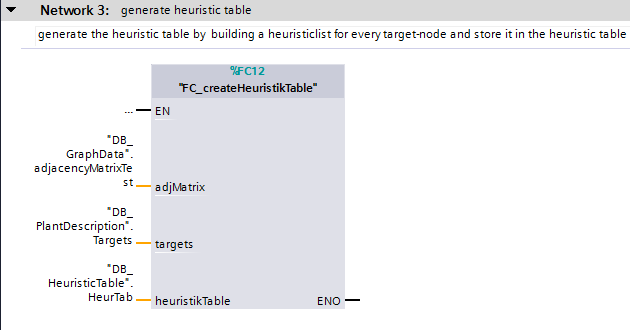
\includegraphics[scale=0.8]{/Bilder/TIA_FC_createHeuristicTable}
				\vspace{0.2cm}
				\caption{Baustein, in dem der Dijkstra-Algorithmus beim Hochfahren der CPU ausgeführt wird.}
				
			\end{figure}
			Der gesamte Dijkstra-Algorithmus\footnote{der Programmcode des den Dijkstra-Algorithmus implementierenden Bausteins ist im Anhang unter \textbf{INSERT REFERENCE HERE} hinterlegt.} wird in einem \ac{FC} mit dem Namen "`FC\_createHeuristicTable"' berechnet \textbf{Insert graphic FC here}. In diesem Baustein wird für jeden Knoten der Anlage aufgerufen, der als Endzielknoten\footnote{vergleiche Abschnitt \ref{Verwendung_Alg}.} markiert ist eine Heuristikliste generiert. Wie bereits erwähnt wird dieser Baustein im "`\ac{OB}100 Startup"' aufgerufen. Die dabei generierten Heuristiklisten werden in einem Datentyp namens Heuristiktabelle in deren Arraykomponente gespeichert und im zyklischen Betrieb von dem A*-Algorithmus verwendet. 
			\\
			\\
			\textbf{Notiz: Bausteine näher beschreiben? mit Auflistung und Erklärung aller Schnittstellen?}
			

		\subsection{A*-Algorithmus}
			\label{Implementierung A*}
			Die Implementierung des A*-Algorithmus ähnelt der des Dijkstra-Algorithmus. Auch hier muss vor Beginn der Berechnung zunächst die Priority-Queue vorbereitet werden. Da der A*-Baustein im Gegensatz zu dem Dijkstra-Baustein mehr als einmal aufgerufen wird,  bedeutet dies, dass die Prioritätsschlange zunächst in den Grundzustand versetzt werden muss, indem alle Knoten aus vorherigen Berechnungen entfernt werden. Zudem muss die Liste der geschlossenen Knoten, die in Abschnitt \ref{A*-Alg} erwähnt wurde, komplett geleert werden, damit kein Knoten bei der Routenberechnung fälschlicherweise als bereits betrachtet angesehen wird.
			\\[4pt]
			Die Berechnung selbst startet nun mit dem Hinzufügen des Startknotens zur Priority-Queue, welche die Liste der offenen Knoten\footnote{Open-List} darstellt. Es wird nun immer der beste Knoten aus der Priority-Queue herausgenommen und als geschlossen markiert. Im Anschluss wird die Adjazenzmatrix nach neuen, vorher nicht erreichbaren Knoten durchsucht. Falls diese noch nicht als geschlossen markiert wurden wird geprüft, ob die Verbindungskante zu dem neuen Knoten in einer speziellen Matrix für permanente Blockaden als blockiert gekennzeichnet wurde. Ist dies nicht der Fall so wird der neue Knoten zu der Liste der offenen Knoten hinzugefügt. Der fertig betrachtete geschlossene Knoten wird dann in die statische Routenliste eingefügt, aus der nach dem Ende der Berechnung die Route generiert wird. Wurde der Zielknoten erreicht oder befinden sich keine Knoten mehr in der Priority-Queue, so beendet sich der Algorithmus. Die Routenliste wird in die Ausgangsvariable kopiert und der Baustein meldet das Berechnungsende über einen Bitmerker an die übergeordnete Wegfindungsschicht.
			\\[4pt]
			Die Erkennung von permanenten Blockaden wurde durch eine Matrix realisiert, da hier, wie auch bei der Adjazenzmatrix, in konstanter Zeit geprüft werden kann ob auf dem betrachteten Streckenabschnitt Behinderungen vorliegen. Diese permanenten Blockaden liegen über längere Zeitintervalle vor und können deshalb bereits zu Beginn der Routenberechnung berücksichtigt werden. Dies ist bei temporären Blockaden durch andere Fahrzeuge nicht der Fall, weshalb zur Erkennung dieser Art von Behinderungen ein anderer Mechanismus zur Anwendung kommt, der in Abschnitt \ref{Kollisionsvermeidung} näher beschrieben wird.
			
		\subsection{Generation der Route}
			\label{Routengeneration}
			Der A*-Algorithmus liefert als Ergebnis eine Liste mit allen geschlossenen Knoten. Aus dieser Liste muss nach Beendigung des Algorithmus eine Route generiert werden, welche in für die Fahrzeugsteuerung verständlicher Form vorliegt. Da die Fahrzeugsteuerungsschicht ebenso wie die Wegfindung über eine Knotenliste der Anlagentopologie verfügt\footnote{wobei für die Fahrzeugsteuerung nur die Verbindungen eines Knotens und nicht die Kantengewichtungen von  Bedeutung sind.}, genügt es, nur eine Liste der KnotenIDs des errechneten kürzesten Pfades zu übertragen.
			\\[4pt]
			Es besteht jedoch das Problem, dass in der Liste der geschlossenen Knoten, auch solche vorkommen können, die nicht Teil des kürzesten Weges sind. Dies ist vor allem dann der Fall, wenn sich die Anlage zwischenzeitlich geändert hat. Würden hier nur die IDs aller Knoten der Liste übertragen, würde dies zu ungültigen Routen für die Fahrteuerung führen, obwohl der Algorithmus einen validen Weg ermittelt hat. Dies ist der Grund, warum die in Abschnitt \ref{Datentypen_Berechnung} vorgestellten Datentypen über die Komponente "`ParentID"' verfügen. Diese hilft bei der Rückverfolgung  des Pfades vom Ziel aus bis zum Startknoten. Um somit eine Route zu generieren, muss zunächst der Zielknoten gefunden werden und dann anhand der ParentIDs der Pfad zum Start einzeln nachverfolgt werden. Der Zielknoten selbst kann einfach gefunden werden, da er mit großer Wahrscheinlichkeit der letzte geschlossene Knoten der Knotenliste ist, da das Erreichen des Ziels eine der Abbruchbedingungen des Algorithmus ist. Die andere Bedingung ist, das keine weiteren Knoten in der Liste der offenen Knoten vorhanden sind. In diesem Fall existiert aber kein Weg vom Start- zum Zielknoten und die Generation der Route ist hinfällig.
			\\[4pt]
			Da die Reihenfolge beim Parsen der Knoten jedoch invers zu der für die Fahrzeugsteuerung benötigten Reihenfolge der Route ist, werden die zum kürzesten Weg gehörenden Knoten temporär in einer Liste abgespeichert, aus der dann durch Umkehrung die eigentliche Route erzeugt wird. Nachdem nun der Zielknoten gefunden wurde, muss mittels der ParentID der vorletzte Knoten der Route gefunden werden. Um nicht auf der Suche nach einem Knoten bei jedem Suchdurchlauf die komplette Knotenliste durchsuchen zu müssen, kann davon ausgegangen werden, dass sich der Vorgänger eines Pfadknotens an einer Stelle in der Liste der geschlossenen Knoten befindet, die vor dem  Index des Pfadknotens liegt. Dies lässt sich gemäß Abschnitt \ref{Dijkstra_Alg} aus der Bedingung für geschlossene Knoten folgern. Bei einer unterschätzenden Heuristik für den A*-Algorithmus wurde für jeden geschlossenen der kürzeste Pfad ausgehend vom Startknoten bereits gefunden. Es ist zudem sinnvoll in absteigender Reihenfolge nach dem Vorgängerknoten zu suchen, da dieser wahrscheinlicher in der Nähe des Pfadknotens selbst zu finden ist als beim Startknoten. Somit kann der Aufwand der Routengeneration auf $\mathcal{O}(n)\le \mathcal{O}(Routengeneration)\ll \mathcal{O}(n^2)$ beschränkt werden.
			
			
	\section{Einhaltung der Echtzeitbedingung}
		\label{Echtzeitbedingung}
		Wenn die Wegfindungsschicht auf der gleichen \ac{SPS} wie die Fahrzeugsteuerungsschicht implementiert wird, so muss die Wegberechnung bestimmte zeitliche Anforderungen erfüllen, damit die Fahrzeugsteuerung nicht beeinträchtigt wird. Eine Steuerung arbeitet im zyklischen Betrieb alle \ac{OB}s nacheinander ab, die als zyklisch definiert wurden. Durch die Modularität des Anwenderprogramms besitzt jede Schicht ihren eigenen zyklischen \ac{OB}, da nur so eine wirkliche Trennung der Schichten möglich ist. Dies bedeutet, dass die Berechnung eines Weges die CPU nicht so lange in Anspruch nehmen darf, dass in dieser Zeit  ein überfahrener RFID-Knoten nicht eingelesen und somit die bevorstehende Kreuzung nicht erkannt wird. Dies führt spätestens beim nächsten erreichten Knoten zu der Erkennung eines Fehlers und das Fahrzeug geht in einen permanenten Fehlerzustand. Ebenso kann es bei zu langer CPU-Belegung vorkommen, dass das Fahrzeug die Spur verliert, dies erst bemerkt wenn es komplett von der Fahrstrecke abgekommen ist und dadurch nicht allein zurück auf die Strecke findet. Aus diesem Grund ist es sehr wichtig, die Wegfindungsschicht so anzupassen, dass zwischen zwei Ausführungen der Fahrzeugsteuerung höchsten 10ms liegen. Da auch die Kommunikationsschichten zyklische \ac{OB}s besitzen, die der Reihenfolge nach abgearbeitet werden müssen, wurde festgelegt, das die Wegberechnung maximal 5ms dauern darf. Dies hat einige Konsequenzen für die Implementierung der Wegfindungsalgorithmen.
		
	
		\subsection{Ausführung bei Systemstart}
			
			Wie bereits mehrfach erwähnt wird die Heuristiktabelle beim Hochfahren der CPU generiert. Eigentlich ist es nicht notwendig für den A*-Algorithmus, dass bereits ein Wert für die Heuristik existiert. Es könnte auch im zyklischen Betrieb ein Wert für die Abschätzungsfunktion $f(n)$ aus Abschnitt \ref{Heuristik} berechnet werden, beispielsweise mittels einer Funktion für die Manhattan-Distanz, welche den Abstand zweier Knoten anhand der Differenz derer Koordinaten ermittelt. Dies würde den Speicherverbrauch erheblich reduzieren, da keine großen Tabellen gespeichert werden müssten, sondern nur die jeweiligen Koordinaten der Knotenpunkte.
			\\[4pt]
			Die Berechnung einer Funktion $f(n)$ ist aber zeitintensiver als das Nachschlagen von Werten in einer Tabelle. Da der Speicherbedarf für die Tabelle der realisierten Anlage mit 25 Knoten und 10 Endzielknoten nur insgesamt 2300 Byte beträgt, fällt dies selbst bei der kleinsten Steuerung vom Typ S7-1214C mit 100kB Arbeitsspeicher kaum ins Gewicht. Zugleich kann die Laufzeit des A*-Algorithmus im zyklischen Betrieb deutlich reduziert werden, da die Tabellenheuristik mittels Dijkstra, im Gegensatz zur Manhatten-Distanz, eine exakte Heuristik liefert, die zusätzlich zur eingesparten Rechenzeit der Tabellenaufrufe noch die Anzahl der betrachteten Knoten minimiert.
			\\[4pt]
			Da die Berechnung des Dijkstra-Algorithmus aber unter anderem auch wegen der gewählten Implementierung mit arraybasierten Priority-Queues zeitintensiv ist \cite{BorisCherkassky1993} und einige Sekunden dauern kann, muss die Tabellengenerierung zu einem Zeitpunkt geschehen, an dem die Echtzeitbedingung der Fahrzeugsteuerungsschicht nicht greift. Aus diesem Grund wurde der Hochfahrvorgang der CPU gewählt, um die notwendigen Initialisierungen der Heuristiktabelle durchzuführen, da hier weder die Fahrzeugsteuerung noch der Watchdogtimer, welcher den zyklischen Betrieb standardmäßig auf 50ms beschränkt, aktiv ist. Zusätzlich wird zu diesem Zeitpunkt noch die Adjazenzmatrix aus der Anlagentopologie generiert, da auch der Parsevorgang der Anlagenknoten bei größeren Anlagen etwas mehr Zeit in Anspruch nehmen kann. Zudem kann somit die Adjazenzmatrix für die schnellere Berechnung des Dijkstra-Algorithmus verwendet werden.
				
		\subsection{Zyklische Ausführung}
			\label{zyklische Auftrennung}
			Trotz der Auslagerung der Heuristikberechnung auf die Hochlaufphase der CPU kann bei langen Routen nicht garantiert werden, das die als Ziel gesetzten 5ms für die Berechnungszeit eingehalten werden. Vor allem wenn sich die Anlage seit dem Hochfahren des Fahrzeugs stark verändert hat und somit die Heuristiktabelle keine exakten Heuristikwerte mehr liefert, müssen unter Umständen zusätzliche Knoten betrachtet werden, die nicht auf dem kürzesten Pfad vom Start- zum Zielknoten liegen. Der Aufwand für die Berechnung verschiebt sich also immer mehr nach $\mathcal{O}(|\mathcal{V}|^2)$ wie in Abschnitt \ref{Aufwand_A*} erläutert wurde.\\
			
			Aus diesem Grund wurde der A*-Algorithmus so implementiert, das der Zeitaufwand pro Zyklus größtenteils konstant bleibt, unabhängig von der Länge der Berechneten Route. Dies wurde erreicht indem die Schleife, welche läuft, solange das Ziel noch nicht erreicht ist, aufgetrennt und durch eine konditionale IF-Abfrage ersetzt wurde. Nach der Schleifenauftrennung wird immer nur ein Knoten pro Zyklus untersucht und gegebenenfalls seine Verbindungsknoten zur Open-List hinzugefügt, weitere Knoten werden erst in den darauf folgenden Zyklen expandiert. Dies hat zur Folge, dass zwar die Bearbeitungszeit pro Zyklus sehr kurz gehalten wird, im implementierten Beispiel wird eine Zykluszeit der Wegfindungsschicht kleiner 1ms erreicht, die Zeit bis zur Berechnung einer kompletten Route jedoch deutlich länger wird. Dies  ist der Fall, da zwischen zwei Bearbeitungszyklen immer die kompletten \ac{OB}s der anderen Schichten abgearbeitet werden. Dieses Problem kann aber zunächst vernachlässigt werden und wird im Abschnitt \ref{Anpassung Kommunikation} näher behandelt.
			\\[4pt]
			Ein zweites Problem, das bei der Aufteilung des Algorithmus auf mehrere Zyklen auftritt, ist die Inkonsistenz von Routen. Während der Berechnung des Algorithmus darf die in Abschnitt \ref{Implementierung A*} erwähnte extern gespeicherte Routenliste nicht als gültige Route missverstanden werden, da hierdurch das Fahrzeug eine möglicherweise falsche Route nehmen würde, die nicht zum Ziel führt. Somit darf der Baustein nur finale Routen ausgeben, und temporäre Routen nur intern speichern. Da der Baustein jedoch in mehreren Zyklen hintereinander aufgerufen wird und zwischen zwei Aufrufen die bereits berechneten Daten nicht verloren gehen dürfen, muss er vom Typ \ac{FB} sein, da nur diese Bausteine einen zugeordneten Instanz-\acl{DB} besitzen, in dem Werte über den Funktionsaufruf hinaus zwischengespeichert werden können.
			\\[4pt]
			Durch die Kombination dieser beiden Maßnahmen, kann erreicht werden, dass die CPU-Belegung durch die Wegfindungsschicht im zyklischen Betrieb, quasi konstant\footnote{immer noch abhängig von der Kantenanzahl des aktuell betrachteten Knotens.} auf unter 1ms gehalten werden kann.
		
	\section{Steuerung des Bearbeitungsablaufs}
		
		Die Wegfindung innerhalb der Anlage besteht nicht allein aus der Berechnung von kürzesten Pfaden zwischen zwei Anlagenknoten. Sie muss auch wissen, welcher Bearbeitungsschritt als nächstes ausgeführt werden soll und welcher Anlagenknoten die korrespondierende Funktionalität besitzt. Zudem soll es möglich sein, dass mehrere Bearbeitungsstationen die gleiche Funktionalität bereitstellen. In diesem Fall muss eine geeignete Station ausgewählt und der Weg zu dem entsprechenden Knoten berechnet werden können.
	
		\subsection{Bearbeitungsreihenfolge}
			\label{Bearbeitungsreihenfolge}
			Im Abschnitt \ref{Aufgabenstellung_Pathfinding} wurde definiert, dass das Fahrzeug selbst die Ablaufreihenfolge der Bearbeitungsschritte kennt. Diese Anforderung wurde durch die Implementierung des Datentyps "`Assignment"' realisiert. Dieser Datentyp stellt eine Art Rezept dar, in dem gespeichert ist, welche Funktionalitäten ein bestimmtes Werkstück benötigt\footnote{Anlagenein- und Ausgänge sind auch Funktionalitäten, die erfasst werden.}. Er ist zusammengesetzt aus der Anzahl der benötigten Funktionalitäten sowie einer Liste der zugehörigen FunktionalitätsIDs. Hierfür muss jedoch zunächst definiert sein, welche Funktionalitäten in der Anlage zur Verfügung gestellt werden und wie die Knoten lauten, die diese Funktionalität bereitstellen. Für diese Aufgabe wurde ein Datentyp erstellt, welcher wie folgt aufgebaut ist:
			
			\begin{table}[h]
				\begin{longtable}{| l | l |}
					
					\hline
					\textbf{FunctionID} & Kennziffer der bereitgestellten Funktionalität.\\ \hline
					\textbf{Nr. of Stations} & Anzahl Stationen, die diese Funktionalität bereitstellen.\\ \hline
					\textbf{Cluster} & KnotenIDs der Stationen, die diese Funktionalität besitzen.\\
					\hline
					
				\end{longtable}
				\vspace{0.2cm}
				\caption{Beschreibung eines Funktionsclusters.}
			\end{table}
			
			Dieses Funktionscluster ermöglicht es nun, Rezepte unabhängig von spezifischen Bearbeitungsstationen zu formulieren. Die Bearbeitungsreihenfolge eines Werkstücks kann somit ausgedrückt werden durch eine Liste aufeinanderfolgender Funktionalitäten, die ein bestimmtes Werkstück benötigt. Im Verlauf der Abarbeitung des Rezepts wählt das Fahrzeug selbst eine der im Cluster hinterlegten Stationen zur benötigten Funktionalität aus. Das Rezept muss der Wegfindungsschicht während des gesamten Bearbeitungsvorgangs zur Verfügung stehen, um die Auswahl des jeweils nächsten Routenziels zu ermöglichen. Daraus folgt, das Rezepte nach der Zuweisung zu einem Werkstück bis zum Abarbeitungsende gespeichert werden müssen.
			\\[4pt]
			Zur Erfassung der Daten von Fahrzeugen, werden die folgenden Informationen gespeichert:
			
			\begin{itemize}
				\item ID des Fahrzeugs, zur Unterscheidung unterschiedlicher Fahrzeuge.
				\item ID des zuletzt besuchten Knotens innerhalb der Anlage.
				\item ID des nächsten Knotens. 
				\item ID des Zielknotens der Aktuellen Route.
				\item Indexnummer des derzeitigen Bearbeitungsschritts innerhalb des zugewiesenen Rezepts.
				\item Das zugewiesene Rezept.
			\end{itemize} 
			
			Für die in Abschnitt \ref{Coop Pathfinding} beschriebene Dynamische Wegfindung ist es notwendig, diese Art von Fahrzeugdaten für alle Fahrzeuge in der Anlage zu speichern. Die ersten drei Punkte sind für alle erfassten Fahrzeuge wichtig, die restlichen Informationen müssen zum derzeitigen Implementierungsstand nur vom eigenen Fahrzeug erfasst werden. Mittels der ID des letzten und des nächsten Knotens kann die Graphenkante identifiziert werden, auf der sich das Fahrzeug momentan befindet. Durch Vergleich des zuletzt besuchten Knotens mit dem Zielknoten der Route wird das Ende der Teilroute erkannt. Auf welchem Weg die benötigten Informationen gesammelt werden, wird im  Kapitel \ref{Kommunikation} näher betrachtet.\textbf{insert graphic of vehiclecontrolblock with assignment here}
			\\[4pt]
			Die Zuweisung von Rezepten erfolgt für jedes Fahrzeug beim Eintritt in die Anlage. Der Anlagenknoten "`0"' stellt in der realisierten Modellanlage den Startknoten dar. Bei Erkennung des Startknotens wird ein Rezept aus der verfügbaren Rezeptliste ausgewählt und dem Fahrzeug zugewiesen. Nach einer kurzen Wartezeit startet die Wegfindungsschicht die Berechnung der Route zur ersten Funktionalität des zugewiesenen Rezepts. Beim Verlassen der Anlage deaktiviert sich die Wegfindung und es wird eine statische Route über die Rückführstrecke zum Anlageneingang zurück gesendet. Beim Erreichen des Eingangsknotens wird erneut ein Rezept zugewiesen. Dies ermöglicht eine endlose Wiederholung des Bearbeitungsvorgangs  mit unterschiedlichen Rezepten bis zum Abbruch durch den Benutzer.
			\\[4pt]
			Ggf für Fazit oder hier: Eine geplante Erweiterung der Anlage sieht vor, dass die Zuweisung von Rezepten durch ein zentrales Steuersystem außerhalb der Anlage abgewickelt wird. Diese Funktion wurde jedoch noch nicht implementiert, weshalb die Zuweisung innerhalb der Wegfindungsschicht stattfindet.
			
		
		\subsection{Zuweisung einer Bearbeitungsstation}
			\label{Zuweisung_Station}
			Existiert pro Funktionalität nur eine Station, so ist die Zuweisung trivial. Existieren aber mehrere Bearbeitungsstation innerhalb eines Funktionalitätsclusters, so muss eine Station ausgewählt werden, welche als Ziel für die nächste Routenberechnung dient. Ein Problem, dass hierbei auftreten kann, ist die ungleichmäßige Auslastung einzelner Bearbeitungsstationen innerhalb eines Clusters. Abbildung \ref{Alternativen} zeigt zwei Stationen mit der gleichen Funktion, wobei sich eine Station näher am Anlageneingang befindet als die zweite. Würden Bearbeitungsstationen nur nach dem Kriterium des kürzesten Weges und des Belegungszustands ausgewählt, so würden alle Fahrzeuge, welche die Anlage betreten, in den meisten Fällen Station 1 anfahren, Station 2 würde nur dann ausgewählt wenn Station 1 belegt ist oder aufgrund von Streckenblockaden der Weg zu Station 2 kürzer ist. Dies würde zu einer verhältnismäßig höheren Auslastung von Bearbeitungsstation 1 führen. Dies ist im industriellen Umfeld jedoch nicht erwünscht, da Anlagenteile meist gleichzeitig modernisiert oder erneuert werden und durch die höhere Auslastung einer Station das Ausfallrisiko dieser Komponente steigt.
			
			\begin{figure}[h]
				\centering
				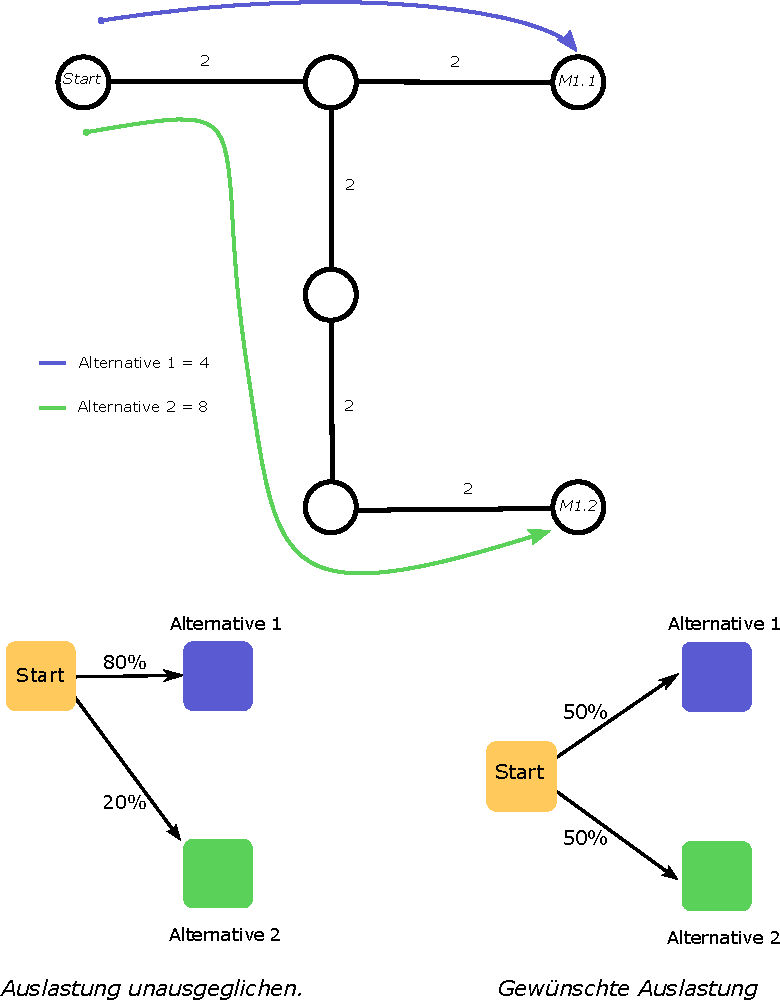
\includegraphics[scale=0.9]{/Bilder/Auslastung_AlternativePDF}
				
				\vspace{0.2cm}
				\caption{Anlage mit zwei Bearbeitungsstationen gleicher Funktionalität}\label{Alternativen}
			\end{figure}
			
		
			Aus diesem Grund wurde entschieden, die Anlagen zufällig an eine der verfügbaren Bearbeitungsstationen des Clusters zu verteilen. Der derzeitige Belegungsstand wurde hierbei vernachlässigt, da die Bearbeitungsdauer einer Station im Modell verglichen mit der Fahrtdauer eines Fahrzeugs sehr gering ist. Somit is eine bei der Berechnung belegte Bearbeitungsstation bis zum tatsächlichen Erreichen der Station wahrscheinlich frei.  Es ergab sich jedoch das Problem, dass unter normalen Umständen Anlagensteuerung exakt arbeiten, da zufällige Ergebnisse innerhalb der Produktion unerwünscht sind. Dies bedeutet das eine \ac{SPS} keinen eingebauten Pseudozufallsgenerator zur Verfügung stellt und dieser somit implementiert werden muss. Zur Generierung von Zufallszahlen wurde hier die Prozessorzeit verwendet, welche durch eine Modulo-Operation mit der Anzahl der zur Auswahl stehenden Bearbeitungsstationen eine für diese Bedürfnisse ausreichende Gleichverteilung der Stationen erreicht.
		
		\subsection{Simulation der Bearbeitungszeit}
			\label{Simulation Station}
			Hat ein Fahrzeug die Bearbeitungsstation am Ende der zugewiesenen Teilroute erreicht, ist es aus Simulationssicht sinnvoll, zunächst ein bestimmtes Zeitintervall zu warten, bevor die nächste Teilroute ausgeführt wird. Hierdurch wird der Bearbeitungsvorgang innerhalb einer Bearbeitungsstation simuliert. Zur Implementierung dieser Funktion wird innerhalb der Wegfindungsschicht bei Erkennen des erreichten Endes einer Teilroute ein Hardwaretimer gestartet, der nach drei Sekunden einen Impuls von einer Periode erzeugt. Dieser Impuls wird verwendet, um die Ausführung der nächsten Teilroute zu starten. Da die Zuweisung von Bearbeitungsstationen wie in Abschnitt \ref{Zuweisung_Station} beschrieben nicht von dem Belegungsstatus der nächsten Zielstation abhängt, kann die Berechnung der nächsten Teilroute bereits während der Simulation des Bearbeitungszustands durchgeführt werden. Durch gerichtete Verbindungen an den Ausgängen der Maschinenplätze ist zudem gewährleistet, das auf der ersten Teilstrecke kein Fahrzeug entgegen kommen kann.
	
		
	\section{Beispiel für eine einfache Routenberechnung}
	
		Das nachfolgende Beispiel zeigt graphisch die Abarbeitung eines einfachen Rezepts mit der Funktionalitätsreihenfolge $(2,1)$. Die Funktionalität 2 wird im vorliegenden Beispiel von den Knoten X und Y bereitgestellt, bei der Funktion 1 handelt es sich um den Ausgang an Knoten 24. Die Funktionalität 0 ist immer den Eingängen zugeordnet, Funktionalität 1 beschreibt analog immer die Ausgänge der Anlage. Es wird angenommen das während der Abarbeitung des Rezepts weder permanente noch temporäre Blockaden auftreten:\\
		\textbf{insert multiple graphics showcasing pathfinding without dynamic reactions here.}
		
	\section{Besonderes Augenmerk bei der generellen Implementierung}
		Bei der technischen Realisierung wurde ein besonderes Augenmerk auf die Effizienz der implementierten Wegfindungsalgorithmen gelegt. Dies wurde teilweise auf Kosten des Speicherbedarfs getan, wie die Implementierung einer exakten Heuristik mittels Dijkstra gut aufzeigt. Trotz allem wurde darauf geachtet, dass die in Kapitel \ref{Anforderungen} definierten Anforderungen bestmöglich erfüllt wurde und somit ein guter Grundstein für den folgenden Schritt der Zusammenführung mit der Fahrzeugsteuerung gelegt wurde. Auch wurde eine Basis geschaffen auf deren Grundlage die im Abschnitt \ref{Coop Pathfinding} beschriebenen Änderungen für eine Kooperative Wegfindung realisiert werden können.